The implementation of the drunk driving simulator is realised with the Unity Engine 3D (Version 2019.4.5f1).
It offers a scripting API in C\#, which is used extensively in the development of the simulation. 
The accessible editor and the built-in asset store allow for quick prototyping with relatively low effort and cost.
The Unity asset store offers a wide variety of content e.g. 3D models, shades, textures, animations etc.
Many third-party assets are used to reduce the development time and create an engaging and visually appealing experience. 
All the used resources are listed and described in sections \ref{subsection:virtual environment}, \ref{subsection:input and physics} and \ref{subsection:visual effects}.
\\
The drunk driving simulator is loosely based on a similar bachelor thesis by \textcite{birgmann2018simulation}.
In this work a virtual reality simulation was developed to show the dangerous implications of distracting factors like using a phone when driving a vehicle.
Some of the assets used are recycled for the simulator in this work and are also listed in the above-mentioned sections.
\\
To simulate alcohol intoxication in VR, this work focuses solely on the effects on human vision and tries to replicate the implications as authentically as possible.
Other negative effects on e.g. balance are not implemented in the drunk driving simulator because of technical limitations and the occurrence of unbearable simulation sickness.
Possible and failed approaches to simulate drunkenness beyond visual effects are established in the discussion section of this work.
In section \ref{subsection:effects of alcohol} commonly observed implications on human abilities are researched and explained.
Section \ref{subsection:visual effects} describes the process on how these effects are implemented into the simulation.
\\
For the purposes of this study some additional logic is implemented to evaluate the behaviour and performance of each driver individually and how the proposed drunk driving simulator is affecting these characteristics.
To acquire usable data the participants of the study have to focus on two separate tasks that are supposed to reliably track their driving performance.
The first assignment is to follow a route along the road and keep the vehicle as close as possible to this path.
In predefined intervals the deviation from the ideal path is measured and logged.
In section \ref{subsection:tracking test} the exact setup of this test is explained.
\\
The second task given to the users is to watch out for potential jaywalkers and react to them by braking and evading if necessary.
This task is used to determine the reaction time of the participant and is elaborated in section \ref{subsection:reaction test}.

\subsection{Virtual Reality}

The virtual reality device used for this project is the Oculus Quest.
The head mounted display (HMD) is designed to provide a wireless VR experience but can also be used in combination with a stationary PC as well.
To use VR in Unity the Steam VR plugin \footnote{https://assetstore.unity.com/packages/tools/integration/steamvr-plugin-32647} has to be integrated into the engine.
The plugin provides a camera setup that can be placed in the scene and is fully functional without any major configurations. 

\subsection{Virtual Environment}
\label{subsection:virtual environment}


When designing the virtual environment several factors are taken into account.
The most important factor are the technical limitations that were present during development.
In his bachelor thesis, \textcite[]{birgmann2018simulation} reported major performance difficulties during the development of the simulation.
The surrounding area was a dense town with many buildings, traffic and other props to enhance the realism.
To meet a consistent and high frame-per-second count many modifications to the objects level of detail and culling properties had to be made that were not ideal.
\\
For the drunk driving simulator another performance concern has to be considered.
Since the drunkenness is mainly achieved through screen shaders that required the software to do additional render passes each frame, the hardware requirements are even higher.
For this reason, an environment with less objects and visual clutter was designed to avoid performance issues. (see figure \ref{figure:overviewEnvironment})
\\
The reason for the more rural appearance of the surroundings is the common traffic situation that is encountered in the place where the study is held.
Near the driving school most roads tend to be curvy and narrow and are surrounded by mostly woods, fields and sparsely populated urban areas.
Most of the study participants are known to be living in this area and are more accommodated to this type of environment.



\begin{figure}[h]
    \centering
	\includegraphics[width=1\linewidth]{images/overviewEnvironment.png}
	\caption[
		Simulator environment overview
	]{
		An overview of the simulator environment.
	}
	\label{figure:overviewEnvironment}
\end{figure}


The buildings scattered in the area are taken from the Town Constructor 3 asset pack. \footnote{https://assetstore.unity.com/packages/3d/environments/urban/town-constructor-3-71070}
It contains a variety of predefined buildings with different level of details that are changed during run-time, depending on the distance to the user camera.
This positively affects the performance since far away objects do not require as much computational power.
The road itself is made with the help of the EasyRoads3D Free v3 asset pack. \footnote{https://assetstore.unity.com/packages/3d/characters/easyroads3d-free-v3-987}
With custom editing tools the road can be easily created and modified and it automatically conforms the terrain to fit accordingly.
The entire track is arranged as a circuit to allow the user to drive multiple laps without a transition.
The terrain and the trees are placed with a built-in Unity functionality.
\\
The vehicle controlled by the user is taken from the realistic car HD 3 asset pack \footnote{https://assetstore.unity.com/packages/3d/vehicles/land/realistic-car-hd-03-113200} and resembles a small sport utility vehicle (SUV) with detailed interior and exterior. 

\subsection{User Input and Physics}
\label{subsection:input and physics}

The input devices used for the simulation is a Logitech G27 steering wheel with a set of pedals. 
With a built-in force feedback mechanism, the steering wheel handles authentically and works with the Unity input system without any issues.
For the physics and control of the vehicle the Realistic Car Controller asset pack \footnote{https://assetstore.unity.com/packages/tools/physics/realistic-car-controller-16296} is used.
The scripts in this pack provide a realistic vehicle control system that handles user input and allows for detailed configuration of the vehicle behaviour.
Most of the settings for the controlled car are taken over from the project of \textcite[]{birgmann2018simulation} since the same input setup was used in this simulation. 


\begin{figure}[h]
    \centering
	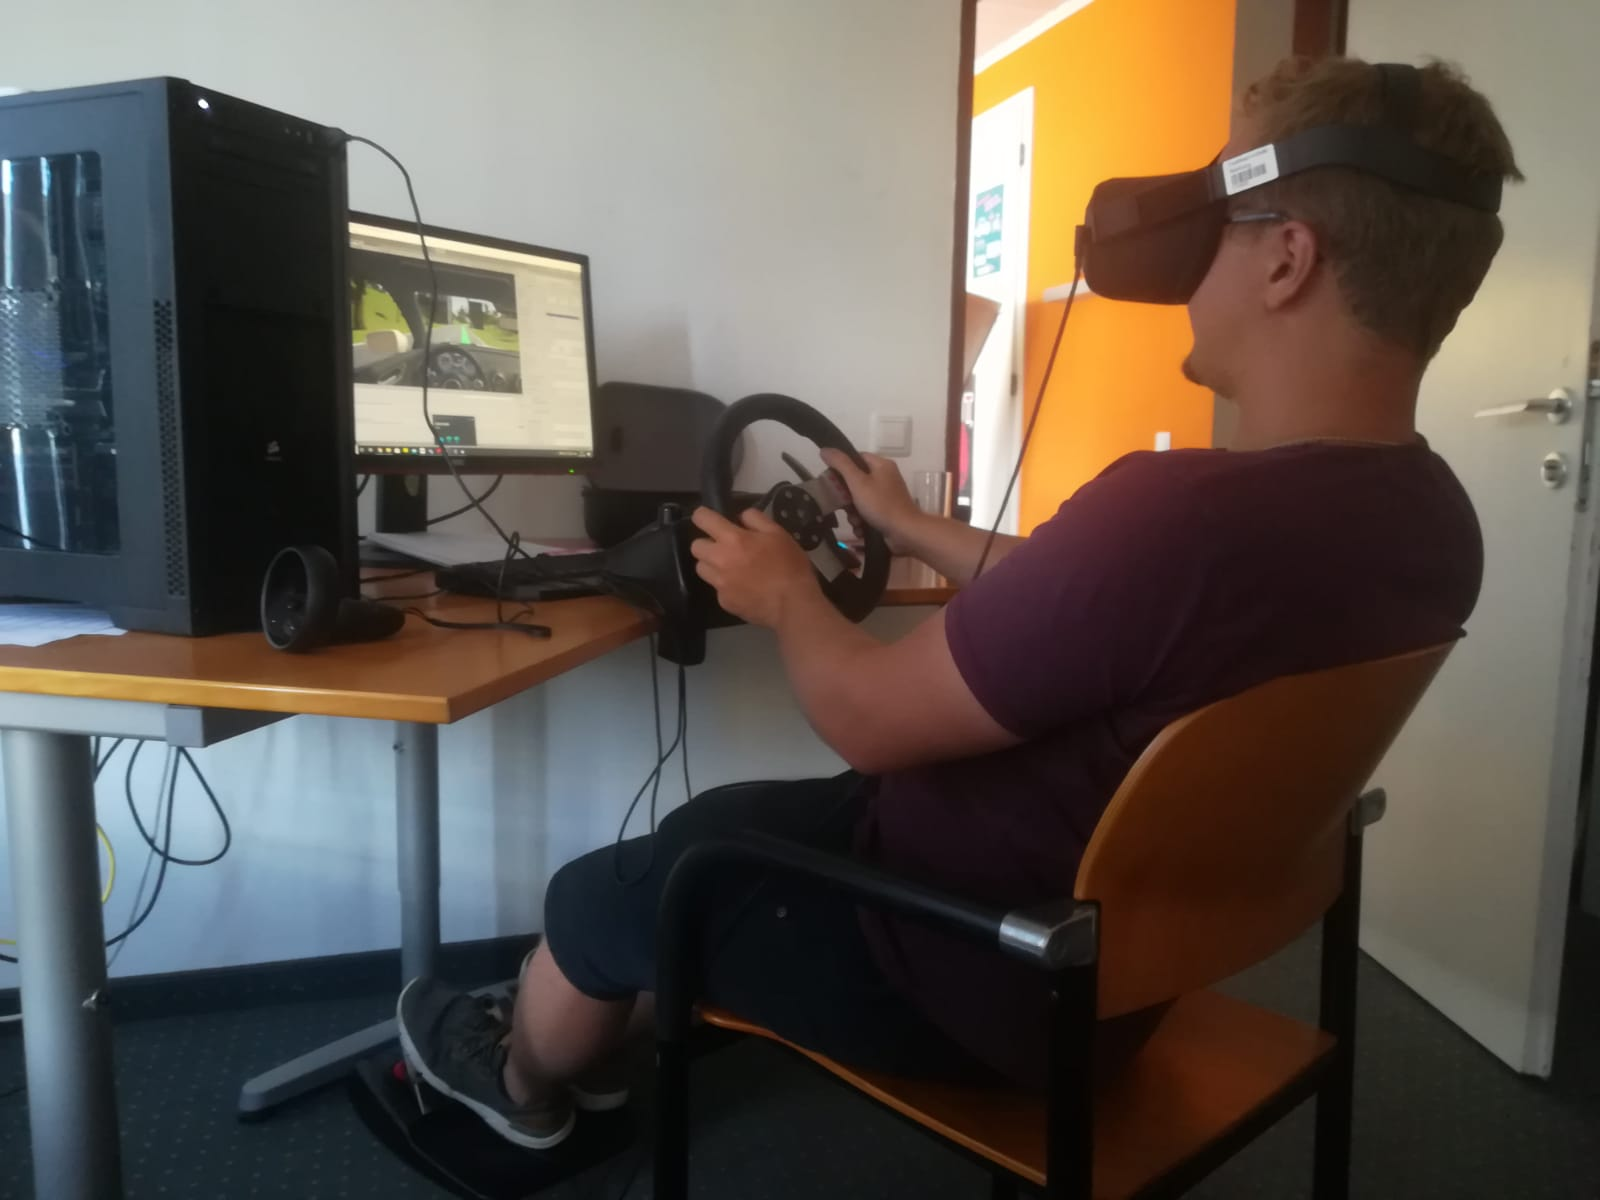
\includegraphics[width=1\linewidth]{images/studySetup.jpeg}
	\caption[
		Simulator setup
	]{
		Setup of the drunk driving simulator.
	}
	\label{figure:overviewEnvironment}
\end{figure}

\subsection{Visual effects}
\label{subsection:visual effects}

To create an authentic drunk experience in the VR simulation the Drunk Man asset pack \footnote{https://assetstore.unity.com/packages/vfx/shaders/fullscreen-camera-effects/drunk-man-47438} is used and modified to fit the needs of the evaluation.
The asset pack includes a camera shader that is supposed to simulate the vision of a drunk person and is generating multiple effects e.g. distortions, color shift, ghost vision etc.
Applying this shader to the camera requires the render pipeline to compute six additional render passes and affects the overall performance and visual quality.
A very noticeable side effect of the shader is the deactivation of anisotropic filtering when viewing the scene in VR.
Anisotropic filtering is supposed to eliminate aliasing effects \autocite{blinn1976texture} and in this case smooth the edges of textures to make their appearance less "blocky".
Even though this does not have implications on the course of the study, improvements on the effects are desirable and are further examined in the discussion section.
\\
Another issue is the amplified occurrence of simulator sickness when applying the shader in VR.
The asset pack is not designed for the use in VR and has to be altered and toned down to make it more tolerable.
To still achieve a decent drunk effect a script is attached to the camera that modifies the shader parameters dynamically according to the behaviour of the user.
To simulate the negative impact on the vergence of the user, the "ghost vision" of the shader is utilized (figure \ref{figure:drunkEffectsIndividual}, top right).
This effect creates a semi-transparent and displaced copy of the screen-image and adds it as an overlay. 
The displacement is controlled over time by a sinus-function and rotates around the centre of the original image.
The severity of this effect is controlled by the rotational movement of the HMD i.e. the more the user moves the head up/down or left/right, the worse the displacement gets.
Not moving the HMD fades out the effect rather quickly. 
To replicate inattentional blindness and alcohol myopia to some degree the "sleepy eye" of the asset pack is modified to act as tunnel vision (figure \ref{figure:drunkEffectsIndividual}, top left).
This creates curved black overlays on the bottom and the top of the screen resembling human eye lids.
Also controlled by the rotational movement of the HMD, if the user does not move the head and just looks straight ahead the tunnel vision effect worsens and severely limits perception.
Moving the head decreases the tunnel vision rapidly but vice versa increases the displacement as mentioned above.
Other effects used is a blur effect that is very subtle on the centre of the screen and increases in severity with less distance to the edges (figure \ref{figure:drunkEffectsIndividual}, bottom right).
This is also intended to simulate alcohol myopia.
A subtle distortion that randomly shifted parts of the image in a radial fashion is not directly used to replicate an effect on vision, but to potentially create a feeling of unease and nausea (figure \ref{figure:drunkEffectsIndividual}, bottom left).
Figure \ref{figure:drunkEffectsCombined} showcases all the combined effects and represents the drunk view used in this simulation.
Note that to prevent simulator sickness the visual effects are toned down and altered continuously, hence the representation in figure \ref{figure:drunkEffectsCombined} is not the final version of the drunk view. 

\begin{figure}[h]
    \centering
	\includegraphics[width=1\linewidth]{images/drunkEffects_individual.png}
	\caption[
		Drunk effects individually
	]{
		The individual effects to achieve drunk vision. Top left - tunnel vision. Top right - image displacement. Bottom left - image distortion. Bottom right - blur effect. 
	}
	\label{figure:drunkEffectsIndividual}
\end{figure}

\begin{figure}[h]
    \centering
	\includegraphics[width=1\linewidth]{images/drunkEffects_combined.png}
	\caption[
		Drunk effects combined
	]{
		The combined effects to achieve drunk vision.
	}
	\label{figure:drunkEffectsCombined}
\end{figure}

\subsection{Tracking test}
\label{subsection:tracking test}
\\
To evaluate the tracking performance of the study participants a predefined path is displayed on the street that should be followed at all times.
On certain points the distance from the car centre to the ideal path is logged to a "comma separated value" (CSV) file.
To realize an exact path layout and distance measurement the BG Curve asset pack\footnote{https://assetstore.unity.com/packages/tools/utilities/bg-curve-59043} is used.
With the tools in this pack a continuous curve can be modelled by hand and fit perfectly to the previously laid out road (see figure \ref{figure:trackingWaypoints}).
Additional mathematical functions are included with the assets that are used to calculate the closest distance from the centre of the car to the curve. (see figure \ref{figure:curveClosestPoint}
In total there are 75 points where the distance to the ideal path is measured.
On straight parts of the road the points are spread out further than in tight curves.
For easier navigation and visibility, the path is highlighted with a green line and the measuring points are visualized with a high transparency sphere mesh.

\begin{figure}[h]
    \centering
	\includegraphics[width=1\linewidth]{images/trackingTestWaypoints.png}
	\caption[
		tracking test way-points
	]{
		The curve and way-points used for measuring the lateral position of the vehicle.
	}
	\label{figure:trackingWaypoints}
\end{figure}

\begin{figure}[h]
    \centering
	\includegraphics[width=1\linewidth]{images/curveClosestPointFunction.jpg}
	\caption[
		curve closest point function
	]{
		Illustration of the closest point function in the BG Curve asset pack.\footnote{http://www.bansheegz.com/BGCurve/DeveloperGuide/Math/}
	}
	\label{figure:curveClosestPoint}
\end{figure}

\subsection{Reaction test}
\label{subsection:reaction test}

For the evaluation in this study one scenario is chosen to resemble a plausible situation in real traffic.
Imitating a jaywalker in an urban environment, a human-like dummy emerges between buildings that are placed very close to the road.
The dummy runs onto the street and stops for a limited time. 
The study participant is advised to brake as soon as the dummy is in line of sight and perform necessary evasive manoeuvres.
This test is triggered multiple times on random places throughout the study and varies in difficulty. 
Even though there are various outcomes for each test instance, for the purposes of this study only the time it takes for the participant to press the brake pedal is measured.
\\
The animated dummy model is taken from the Basic Motion FREE Pack. \footnote{https://assetstore.unity.com/packages/3d/animations/basic-motions-free-pack-154271}
With a short script and the use of the unity rag-doll system the dummy reacts physically plausible when hit by a vehicle.
Even though this does not have further implications on the test procedure, every crash with the dummy is noted down during the experiment.
During testing it was observed that a human-like dummy crashing into the windshield of the car tends to have an unsettling impact on the driver, which is the main reason why a crash dummy was used instead of a model of a real person. 
\begin{figure}[h]
    \centering
	\includegraphics[width=1\linewidth]{images/reactionTestLOSCheck.png}
	\caption[
		Reaction test LOS check
	]{
		Checking the line of sight to the dummy directly from the driver camera. 
	}
	\label{figure:LOSCheck}
\end{figure}
A large trigger is placed on the road to determine if the user is approaching the dummy that is still hidden out of sight.
On entering the trigger, the velocity of the car and its distance to the potential crash point is tracked to determine how much time it takes the vehicle to reach the crash spot (time = distance/velocity).
The dummy follows the same logic and as soon as the car reaches a critical time left to the crash point, the dummy starts approaching said spot.
This logic requires the user to react in a limited time frame and creates equal circumstances for slow and fast drivers.
\\
As soon as the dummy starts moving a continuous line of sight check from the user camera to the dummy is performed. (see figure \ref{figure:LOSCheck})
The test logs the exact time to a CSV file when a potential line of sight is given.
At this point the driver is able to see the jaywalker approaching the street and should react by pressing the brake.
During this time window the test logs the moment it receives a braking input i.e. the moment the brake pedal is pushed in even slightly. 
This allows for relative freedom where and how the test is placed and provides accurate reaction times.
\\
For the experiment six instances of the reaction test are placed over the entire track and during each lap three randomly chosen tests are active.


